\documentclass{standalone}
\usepackage{fontspec}
\usepackage[dvipsnames]{xcolor}
\usepackage{tikz}

\begin{document}
\begin{tikzpicture}
\clip (-3\textwidth/4, 0.5in) -- (3\textwidth/4, 0.5in) -- (3\textwidth/4, -0.5in) -- (-3\textwidth/4, -0.5in) -- cycle;

\node[fill=Blue, inner sep=0.4cm, minimum width=2\textwidth] at (0,0) {\setmainfont[Scale=3.0]{Chakra Petch-Bold}\Huge \textcolor{Goldenrod}{PING}};

\node[circle, minimum width=2.0in, fill=Goldenrod, opacity=1, inner sep=0pt] at (-2.375in, 0) {};
\node[circle, minimum width=1.75in, fill=Blue] at (-2.375in, 0) {};
\node[circle, minimum width=1.5in, fill=Goldenrod, opacity=1] at (-2.375in, 0) {};
\node[circle, minimum width=1.25in, fill=Blue] at (-2.375in, 0) {};
\node[circle, minimum width=1.0in, fill=Goldenrod, opacity=1] at (-2.375in, 0) {};
\node[circle, minimum width=0.75in, fill=Blue] at (-2.375in, 0) {};
\node[circle, minimum width=0.5in, fill=Goldenrod, opacity=1] at (-2.375in, 0) {};
\node[circle, minimum width=0.25in, fill=Blue] at (-2.375in, 0) {};

\node[circle, minimum width=2.0in, fill=Goldenrod, opacity=1] at (2.375in, 0) {};
\node[circle, minimum width=1.75in, fill=Blue] at (2.375in, 0) {};
\node[circle, minimum width=1.5in, fill=Goldenrod, opacity=1] at (2.375in, 0) {};
\node[circle, minimum width=1.25in, fill=Blue] at (2.375in, 0) {};
\node[circle, minimum width=1.0in, fill=Goldenrod] at (2.375in, 0) {};
\node[circle, minimum width=0.75in, fill=Blue] at (2.375in, 0) {};
\node[circle, minimum width=0.5in, fill=Goldenrod] at (2.375in, 0) {};
\node[circle, minimum width=0.25in, fill=Blue] at (2.375in, 0) {};

\node at (-2.375in, 0) {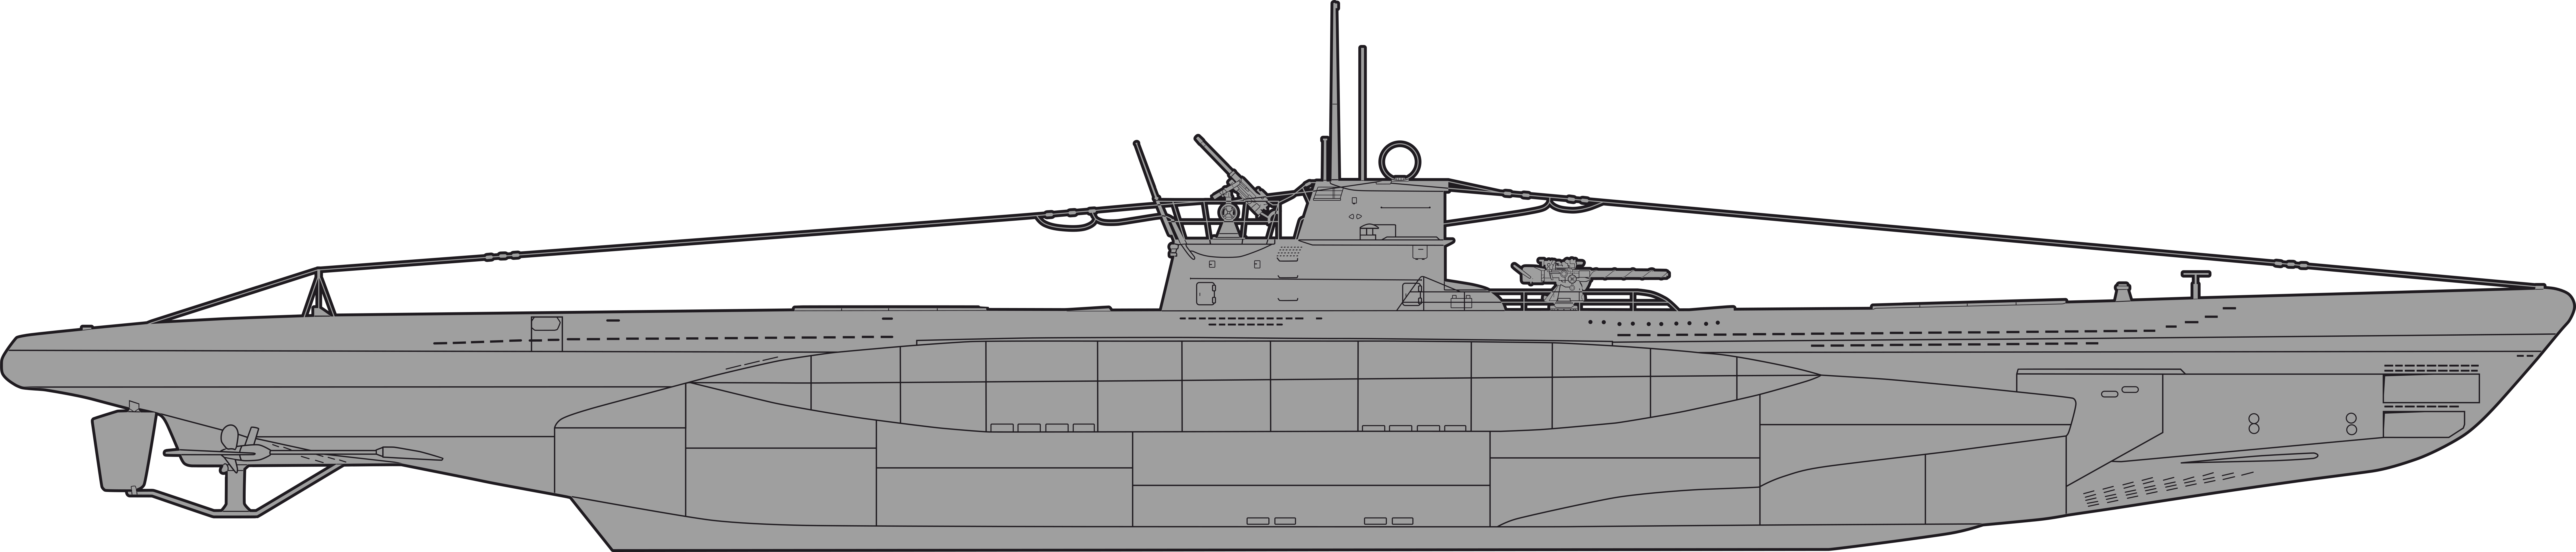
\includegraphics[height=0.425in]{uboat_dark.png}};
\node[xscale=-1] at (2.375in, 0) {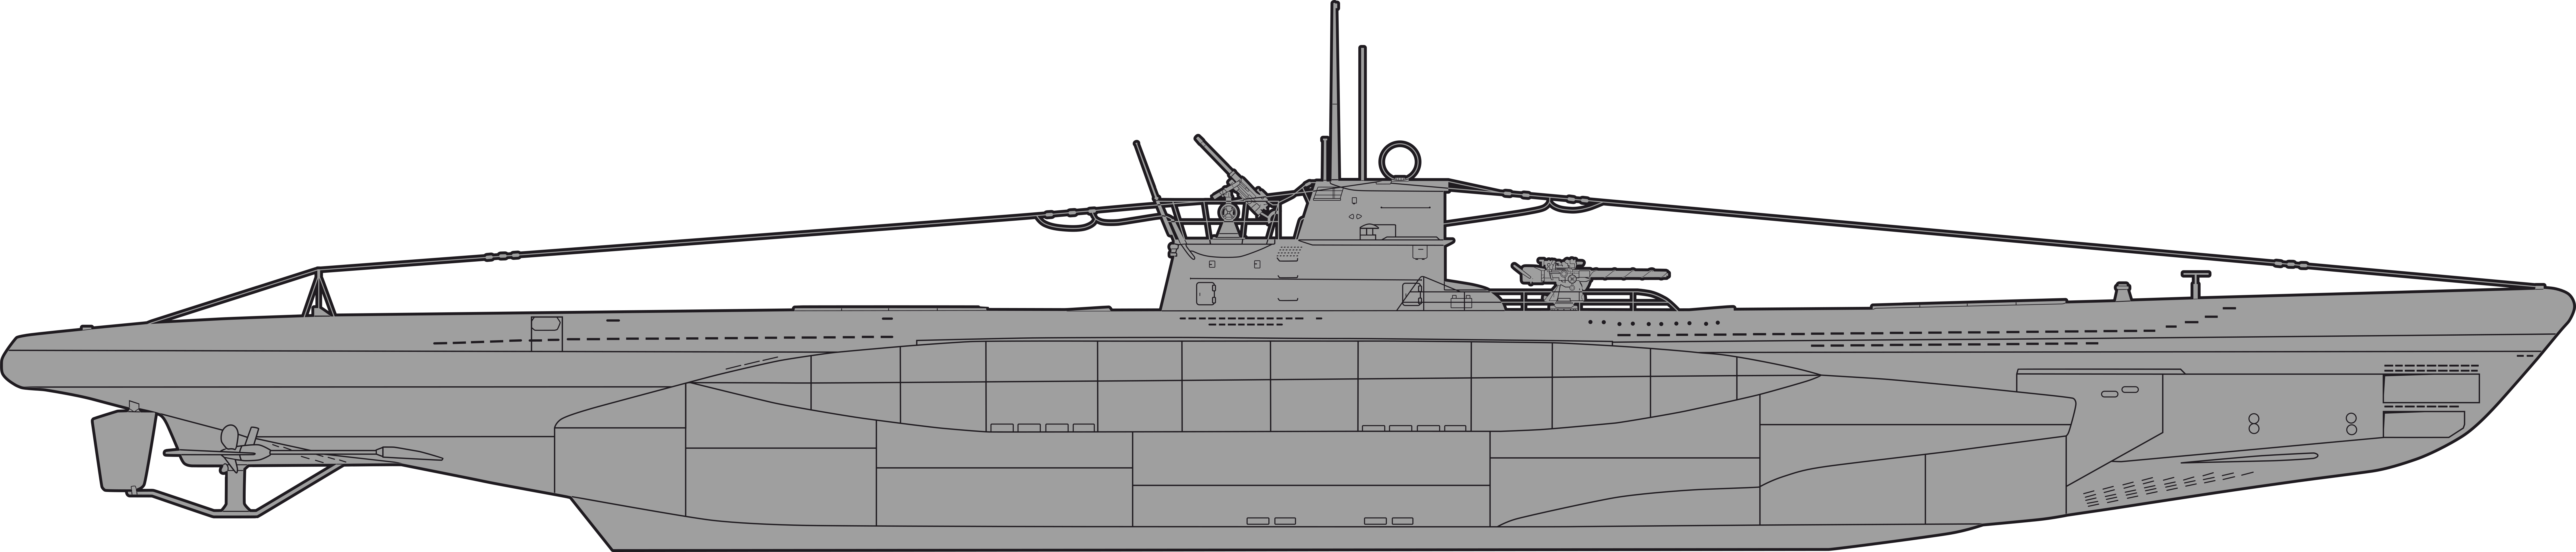
\includegraphics[height=0.425in]{uboat_dark.png}};
\end{tikzpicture}


\end{document}